\chapter{ARMA}
\label{chap:arma}
\section{Some Definitions}
Let's give some definitions:
\begin{itemize}
	\item Stocastic process (univariate): sequence of random variables $Y_t$
	\item Second order process: $\mathbf{E}[Y_t^2] < + \infty \ \forall t$
	\item Mean $\mu_t = \mathbf{E}[Y_t]$ and variance $\sigma^2 = \mathbf{E}(Y_t - \mu_t)^2$
	\item Autocovariance $\gamma_t(k) \equiv Cov(Y_t,Y_{t-k}) = \mathbf{E}[Y_t - \mu_t][Y_{t-k} - \mu_{t-k}]$, from this we can define $\sigma^2_t = \gamma_t(0)$
	\item Autocorrelation:
	\[
	\rho_t(k) \equiv Corr(Y_t,Y_{t-k}) = \frac{\gamma_t(k)}{\sqrt{\gamma_k(0) \gamma_{t-k}(0)}}
	\]
\end{itemize}
We give some definitions of stationarity:
\begin{mydefinition}[Strict stationarity]
\begin{equation}
	(Y_1,\ldots, Y_n) \stackrel{d}{=} (Y_{1+k},\ldots, Y_{n+k}) \quad \forall n>1,k
\end{equation}
we use $\stackrel{d}{=}$ as converges in distribution.
\end{mydefinition}
\newpage
\begin{mydefinition}[Weak/second-order/covariance stationarity]
Under this conditions:
\begin{itemize}
	\item $\expected{Y_t} = \mu$ 
	\item $\expected{Y_t -\mu}^2 = \sigma^2 < +\infty$
	\item $\mathbf{E}[Y_t - \mu_t][Y_{t-k} - \mu_{t-k}] = \gamma(|k|)$ (independent of $t$ for each $k$)
	than:
	\begin{equation}
	\rho(k) = \frac{\gamma(k)}{\gamma(0)}
	\end{equation}
\end{itemize}
This is the most common definition of stationarity
\end{mydefinition}

\begin{mydefinition}[Ergodicity]
We consider three different definition:
\begin{itemize}
	\item In mean: $\bar{y} \equiv \frac{1}{T} \sum_{t+1}^{T} Y_t \xrightarrow{p} \gamma(k)$
	\item In second moments: $\frac{1}{T} \sum_{t+1}^{T} (Y_t - \mu) (Y_{t-k} - \mu) \xrightarrow{p} \gamma(k)$
	\item if a stationary process $Y_t$ satisfy $\sum_{k=0}^{+ \infty} |\gamma(k) <\infty$ then $Y_t$ is ergodic in mean.\\
\end{itemize} 
This one is less used 
\end{mydefinition}
We can give this intepretations:
\begin{itemize}
	\item uncodintional mean and variance are constant.
	\item mean reversion
	\item shocks are transient
	\item covariance between $Y_t$ and $Y_{t-k}$ tends to 0 if $k \to \infty$
\end{itemize}
\newpage
We define white noise as:
\begin{mydefinition}[Weak (uncorrelated)]
	\begin{itemize}
		\item $\expected{\epsilon_t} = 0 \ \forall t$
		\item $Var(\epsilon_t) = \sigma^2 \ \forall t $
		\item $Corr(\epsilon_t, \epsilon_s) = 0 \ \forall s \neq t$
	\end{itemize}
\end{mydefinition}

\begin{mydefinition}[Strong (independece)]
	$\epsilon_t \sim i.i.d(0,\sigma^2)$
\end{mydefinition}

\begin{mydefinition}[ Gaussian (weak = strong)]
		$\epsilon_t \sim n.i.d (0, \sigma^2)$ (if uncorrelated, than are independent)
\end{mydefinition}
Introducing the lag operator proves advantageous to furthers discussions:

\begin{mydefinition}[Lag operator ]
The lag operator is defined as:
\begin{equation}
	LY_t \equiv Y_{t-1}
\end{equation}
\end{mydefinition}
Some properties of lag operator:
\begin{itemize}
	\item it is a linear operator:
	\[
	L(\alpha X_t + \beta Y_t) = \alpha L(X_t) + \beta L(Y_t) = \alpha X_{t-1} + \beta Y_{t-1}
	\]
	\item it admits power exponent:
	\begin{align*}
		&L^k Y_t = Y_{t-k}\\
		& L^{-k} Y_t = Y_{t+k}
	\end{align*}
\end{itemize}
Using lag operator we can define:
\begin{align*}
	&\text{First diffent}:  & \Delta Y_t = Y_t - Y_{t-1} = Y_t - LY_t = (1-L)Y_t\\
	&AR(2): & Y_t = \theta_1 Y_{t-1} + \theta_2 Y_{t-2} = (\theta_1 L + \theta_2 L^2)Y_t
\end{align*}
A lag polynomial $\theta(L)$ is:
\[
L(\theta) = \sum_{k = 0}^{+\infty} \theta_kL^k
\]
\section{Moving Avarage (MA) process}
Lag operator is useful to costruct a stationary process. For example we cas costruct a sort of weighted moving average of white noise $\epsilon_t$: 
\begin{mydefinition}[MA(q)]
\begin{equation}
	\mathrm{MA(q)}: Y_t = \theta(L)\epsilon_t = \epsilon_t + \theta_1\epsilon_{t-1} + \ldots + \theta_q\epsilon_{t-q}
	\label{MA}
\end{equation}
\end{mydefinition}
It is useful studying the first order understand MA(q) structure:
\[
\mathrm{MA(1)}: Y_t = \epsilon_t + \theta \epsilon_{t-1} = (1 + \theta L)\epsilon_t
\]
If we study the expected value and covariance:
\begin{align*}
	\expected{Y_t} &= 0 \\
	\gamma(0) &= \expected{Y_tY_t} = \ldots = \sigma^2(1 + \theta^2)\\
	\gamma(1) & = \expected{Y_tY_{t-1}} = \ldots = \sigma^2 \theta\\
	\gamma(k) & = \expected{Y_tY_{t-k}} = \ldots = 0\quad \forall k>1
\end{align*}
so that:
\begin{align}
	\rho(1) &= \frac{\gamma(1)}{\gamma(0)} = \frac{\theta}{1 + \theta^2}&\\
	\rho(k) &= \frac{\gamma(k)}{\gamma(0)} = 0 \qquad  \forall k>1
\end{align}
While white noise is 0-correlated, MA(1) is 1-correlated, this means that only the first correlation is different from zero. The first correlation is easy to evaluate and measuring. So that if we noticed that some samples have only the first correlation different from zero, it could come from a MA(1).\\
We can generalize it for MA(q):
\begin{align}
	\gamma(0) & =\sigma^2(1 + \theta_1^2 + \ldots + \theta^2_q)&\\
	\gamma(k) & = \sigma^2\sum_{j=0}^{q-k} \theta_j\theta_{j+k} & \forall k \leq q\\
	& = 0 & \forall k > q
\end{align}
MA(q) is q-correlated and any stationary q-correlated process can be represented as an MA(q).\\
At same time MA(q) process is not unique, but there is only one MA(q) that is invertible.\\
As early, we can study MA(1) and than generalize: given $Y_t = (1 + \theta L)\epsilon_t$ we can expand it in a Taylor series:
\[
(1 + \theta L)^{-1} = (1 - \theta L + \theta^2 L^2 + \ldots)= \sum_{i = 0}^{+ \infty} (-\theta L )^i
\]
inverting the $\theta(L)$ lag polynomial:
\[
(1 - \theta L + \theta^2 L^2 + \ldots)Y_t = \epsilon_t
\]
which is AR$(\infty)$.\\
If an MA process can be written as AR$(\infty)$, than MA process is invertible.\\
For MA(1) process, the invertibility is given by $|\theta| < 1$.
Generalizing it, a MA(q)  process is invertible if the roots of the lag polynomial:
\[
1 + \theta_1 z + \ldots + \theta_q z^q = 0
\]
lie outside the unit circle.\\
Invertible has an important practical in application: given $\epsilon_t$ a non observable, it could be reconstructed from $Y$ through a AR$(\infty)$ representation.
Let's make an example: given the generic lag polynomial:
\[
\theta(L) = 1 + \theta_1 L + \theta_2 L^2 + \ldots + \theta_qL^q
\]
we have to find the series $\theta(L)^{-1} = \varphi_0 + \varphi_1L + \ldots$ such that:
\[
(1 + \theta_1 L + \theta_2 L^2 + \ldots + \theta_qL^q)(\varphi_0 + \varphi_1L + \varphi_1L^2\ldots) = 1
\]
coefficients $\varphi_i$ can be computed recursively matching $L^k$ (easy to compute)
\section{Auto-Regressive Process (AR)}
A general AR process is defined as:
\begin{equation}
	\phi(L)Y_t = \epsilon_t
	\label{AR}
\end{equation}

Analysing AR(1):
\[
(1- \phi L)Y_t = \epsilon \quad \text{or} \quad Y_t = \phi Y_{t-1} + \epsilon_t
\] 
inverting the lag polynomial $(1- \phi L)$ the AR(1) can be written as:
\[
Y_t = (1- \phi L)^{-1}\epsilon_t = \sum_{i=0}^{\infty} (\phi L)^i = \sum_{i = 0}^\infty \phi\epsilon_{t-i} = \text{MA}(\infty)
\]
stationary condition is $|\phi| < 1$\\.
From this represention, we can compute $\rho(\cdot)$:
\[
\rho(k) = \phi^{|k|} \quad \forall k 
\]
\newpage
In general AR(p) process is define as:
\begin{mydefinition}[AR(p)]
	\begin{equation}
		\text{AR(p)}: Y_t = \phi_1Y_{t-1} + \phi_2Y_{t-2} + \ldots + \phi_p Y_{t-p} + \epsilon_t
	\end{equation}
\end{mydefinition}
AR(p) is stationarity if all roots of the characteristic equation of lag polynomial:
\[
1 - \phi_1Z - \phi_2z^2 - \ldots - \phi_pz^p=0
\]
are outside of unite circle.\\
Exposing AR(p) in its state space from:
\begin{equation*}
	\begin{bmatrix}
		Y_t \\
		Y_{t-1}\\
		\vdots\\
		Y_{t-p+1}
	\end{bmatrix} =
\begin{bmatrix}
	\phi_1 & \phi_2 & \cdots & \phi_{p-1} & \phi_p \\
	1 & 0 & \cdots & 0 & 0\\
	\vdots & \vdots & \cdots & \vdots & \vdots\\
	0 & 0 &\cdots &1 & 0\\
\end{bmatrix}
	\begin{bmatrix}
	Y_{t-1} \\
	Y_{t-2}\\
	\vdots\\
	Y_{t-p}
\end{bmatrix}
+
	\begin{bmatrix}
	\epsilon_t \\
	0\\
	\vdots\\
	0
\end{bmatrix}
\end{equation*}
It can be expresses as:
\[
X_t = F X_{t-1} + v_t
\]
The expected value of $X_t$ satisfy:
\[
\expected{X_t} = F X_{t-1}\quad \text{and} \quad \expected{X_{t+j}} = F^{j +1}X_{t-1}
\]
whose dynamic is given by the eigenvalues of the matrix $F$

\section{Partial Autocorrelation Function (PACF)}
For an AR(p) process, the $k$-lag ACF $\rho_k$ can be interpreted as simple regression:
\[
Y_t = \rho_k Y_{t-k} + \text{error}
\]
and the $k$-lag PACF:
\[
a_t(k) \equiv Corr(Y_t, Y_{t-k} | Y_{t-1}, \ldots, Y_{t-k+1})
\]
can be build as multiple regression:
\[
Y_t = a_1 Y_{t-1} + a_2 Y_{t-2} + \ldots + a_kY_{t-k} + \textbf{error}
\]
that can be computed by solvig the Yule-Walker system:
\begin{equation*}
	\begin{bmatrix}
		a_1 \\
		a_2\\
		\vdots\\
		a_k
	\end{bmatrix} =
	\begin{bmatrix}
		\gamma(0) & \gamma(1) & \cdots & \gamma(k-1) \\
		\gamma(1) & \gamma(2) & \cdots & \gamma(k-2)\\
		\vdots & \vdots & \cdots & \vdots \\
		\gamma(k-1) & \gamma(k-2) & \cdots & \gamma(0)\\
	\end{bmatrix}^{-1}
	\begin{bmatrix}
		\gamma(1) \\
		\gamma(2)\\
		\vdots\\
		\gamma(k)
	\end{bmatrix}
\end{equation*}
We can conclude that AR(p) process are p-partially correlated. That is a useful tool to identify AR order
\begin{center}
	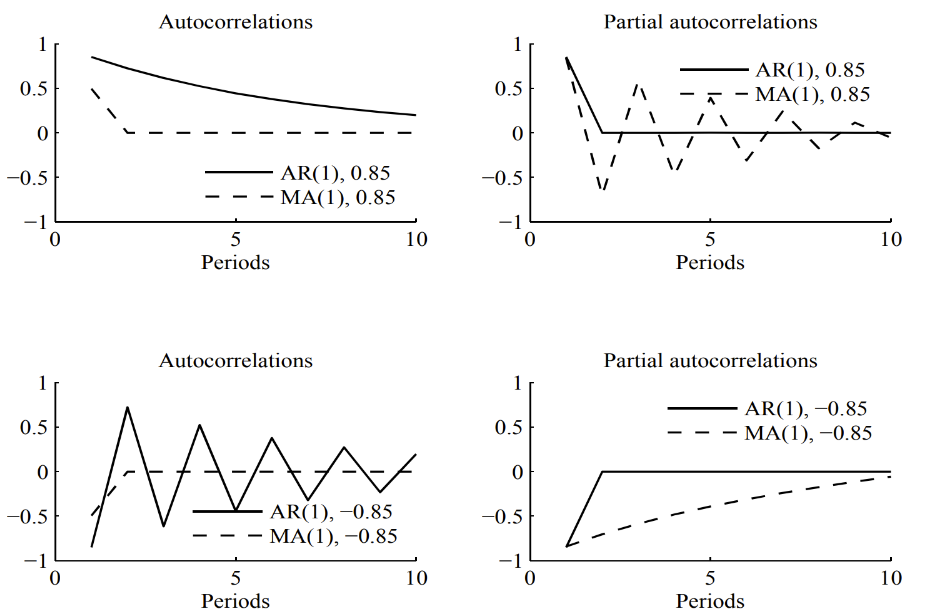
\includegraphics[width=0.5\textwidth]{picture/(1)autocorrelation.png}
\end{center}
\section{ARMA(p,q)}
An ARMA(p,q) process is defined as
\begin{mydefinition}[ARMA]
	\begin{equation}
	\phi(L) Y_t = \theta(L) \epsilon_t
\end{equation}
\end{mydefinition}

where $\phi(L)$ and $\theta(L)$ are $p^{th}$ and $q^{th}$ lag polynomials.\\
Process is stationary if all the roots of polynomial:
\[
\phi(z) \equiv 1 - \phi_1 z - \phi_2 z^2 - \ldots - \phi_{p-1}z^{p-1} - \phi_pz^p = 0
\]
lie outside the unit circle $\rightarrow$ admits MA($\infty$) representation:
\[
Y_t = \phi(L)^{-1} \theta(L)\epsilon_t
\]
The process is invertible if all roots of
\[
\theta(z) \equiv 1 + \theta_1 z + \theta_2 z^2 + \ldots + \theta_{q-1}z^{1-1} + \theta_qz^q = 0
\]
lie outside the unit circle $\rightarrow$ admits AR($\infty$) representation:
\[
\epsilon_t = \theta(L)^{-1} \phi(L)Y_t
\]
\section{Estimate AR models}
In time series the data are usually not i.i.d, so that it is better use prediction-error decomposition of likelihood:
\[
L(y_T,y_{T-1},\ldots,y_1;\theta) = f(y_T | \Omega_{T-1};\theta) \cdot f(y_{T-1}| \Omega_{T-2};\theta)\cdot \ldots \cdot f(y_{1}| \Omega_{0};\theta)
\]
Let's make an example for AR(1) (gaussian noise): 
\[
y_t = \phi_1 y_{t-1} + \epsilon_t
\]

the full log-Likelihood is:
\[
I(\phi) = \underbrace{f_{Y_1}}_{\text{marginal } 1^{\text{st}} \text{ obs}} (y_1;\phi) +   \underbrace{\sum_{t=2}^T f_{Y_t|Y_{t-1}}(y_t|y_{t-1};\phi)}_{\substack{\text{conditional likelihhod} \\ \text{under normality OLS = MLE}\\ \text{process AR(1), it is Markovian}}} = f_{Y_1}(y_1;\phi) - \frac{T}{2} \log (2 \pi) - \sum_{t =1}^{T} \log \sigma^2 - \frac{1}{2} \sum_{t=1}^T \frac{(y_t - \phi y_{t-1})^2}{\sigma^2}
\]
Maximing conditional likelihood for $\phi \rightarrow$ minimize:
\[
\sum_{t=2}^T (y_t - \phi y_{t-1})^2
\] 
In general AR(p) process under gaussianity are asymptotically equivalent to MLE.
\section{Estimation MA models}
Let's consider MA(1):
\[
y_t = \theta \epsilon_{t-1} + \epsilon_t
\]
The full log-Likelihood is:
\[
I(\phi) = \underbrace{f_{Y_1}}_{\text{marginal } 1^{\text{st}} \text{ obs}} (y_1;\phi) +   \underbrace{\sum_{t=2}^T f_{Y_t|Y_{t-1}}(y_t|y_{t-1};\phi)}_{\text{conditional likelihhod}} = f_{Y_1}(y_1;\phi) - \frac{T}{2} \log (2 \pi) - \sum_{t =1}^{T} \log \sigma^2 - \frac{1}{2} \sum_{t=1}^T \frac{(y_t - \epsilon y_{t-1})^2}{\sigma^2}
\]
$\epsilon$ are not observed, I observe $y$, $\epsilon$ can be recover from $y$:
\[
\epsilon_t = y_t - \theta \epsilon_{t-1} = (- \theta)^t \epsilon_0 + \sum_{i = 1}^{t} (-\theta)^i y_{t-i}
\]
if MA is invertible; minimaztion of RSS is non-linear in $\theta$, we need MLE or Non-Linear Least Square
\section{Estimate ARMA models}
For general ARMA(p,q):
\[
T_t = \phi_1Y_{t-1} + \ldots + \phi_p Y_{t-p} + \epsilon_t + \theta_1 \epsilon_{t-1} + \ldots \epsilon_q
\epsilon_{t-q}\]
$Y_{t-1}$ is correlated with $\epsilon_{t-1},\ldots, \epsilon_{t-q}$, so $\expected{ \epsilon | X} \neq 0$, OLS is not onsistent. We need MLE with numerical optimization procedures.

\section{Optimal Prediction}
\begin{mytheorem}[Optimal Prediction]
	If the Loss function of a prediction is a quadratic function of the prediction error i.e, the MSE:
	\[
	MSE(\hat{Y}_t)\equiv \expected{Y_t - \hat{Y}_t}^2
	\]
Than the optimal prediction of $Y$ in terms of past values $X$ is given by conditional expectation $\expected{Y_{t+1}|X_t}$
\end{mytheorem}
If process $Y$ is linear or normally distributed, linear projection: $\hat{Y}_t \equiv P (Y_{t+1}| X_t) = \alpha 'X$ is the optimal prediction, $\alpha' = [\expected{X_tX'_t}]^{-1}\expected{X'_t Y_{t+1}} \simeq OLS$.\\
In general:

\[
Y_{t+k} = \underbrace{\text{function of past values}}_{\text{determine } \expected{Y_{t+k}}} + \underbrace{\text{fucntion of future values}}_{\text{determine} Var_t(Y_{t+k})}
\]
\section{Wold Theorem}
\begin{mytheorem}[Wold Theorem]
	Any mean zero covariance stationary process can be represented in the form:
	\begin{equation}
			Y_t =  \underbrace{\sum_{j=0}^\infty \varphi_j \epsilon_{t-j}}_{\text{random}} + \underbrace{k_j}_{\text{deterministic}}
			\label{wold_theorem}
	\end{equation}
where:
\begin{itemize}
	\item $\sum_{j=0}^{\infty} \varphi_j^2 < \infty, \varphi_0 =1$
	\item $\epsilon_t = Y_t - P(Y_t | Y_{t-1}, Y_{t-2}, \ldots)$ are linear prediction errors
	\item $\{\varphi_j\}, \{\epsilon_j\}$ are unique
	\item $k_j$ is linearly deterministic
	\item $\epsilon_{t-j}, k_j$ are uncorrelated.
\end{itemize}
\end{mytheorem}
\section{Box-Jenkins Approach}
Box-Jenkins Approach is a standard procedure models to find the best fit of a time-series model to past values of a time series.
\begin{itemize}
	\item First of all check for stationarity (exists some statistical test), if it fails, try transformation.
	\item Identification: check autocorrelation function (MA(q) model are q-correlated process) and partial autocorrelation function (AR(p) are p-partially correlated process) 
	\item Validation: checl appropriateness of the model by some measure of fit (AIC/Akaike, Bic/Schwarz, residua,...)
\end{itemize}
\section{ARIMA}
ARIMA model is an integrated ARMA model. ARIMA(p,1,q) denote a nonstationary process $Y_t$ for which the first difference is an ARMA(p,q) process:
\begin{mydefinition}[ARIMA(p,1,q)]
		\begin{equation}
		Y_t - Y_{t-1} = (1-L)Y_t
	\end{equation}
\label{ARIMA}
\end{mydefinition}
$Y_t$ is siad to be intefrated of order 1 ($I(1)$)\\
$I(2) \rightarrow Y_t$ is integrated of order 2 if : $Y_{t} - Y_{t-1} = (1-L)^2Y_t$
\section{ARFIMA}
We can try to think on a difference operator and ask what is the meaning of a Lag-operator with exponent fractional.\\
The $k-$ difference operator $(1-L)^n$ with integer $n$ can be generalized to a fractional operator $(1-L)^d$ with $0<d<1$ defined by the binomial expansion:
\[
(1-L)^d = 1 -dL + d(d-1)L^2/2! + \ldots
\]
If $d< 0.05$, the process is cov stationary and admits an AR($\infty$) representation.\\
Fractional filter $(1-L)^d$ produces hyperbolic decaying autocorrelation, the so colled long memory. for ARFIMA(pd,q) processes:
\[
\phi(L) (1-L)^dY_t = \theta(L)\epsilon_t
\]
its autocrrelation functions is proportional to:
\[
\rho(k) \simeq ck^{2d -1}
\]